%.-------------------------------------------------------------------------------------------------------------------------------------------------------------
\subsection{Install Java}
If you already have the latest version of java sdk skip this step.
Visit the \href{https://www.oracle.com/technetwork/java/javase/downloads/jdk13-downloads-5672538.html}{jdk installation page}.
Accept license agreement and install the version suitable for your operating system.
If you downloaded the executable execute it if you downloaded the zip version unzip it in a new directory called JAVA which you should place in the programs folder of your pc. 
\begin{figure}[h]
\centering
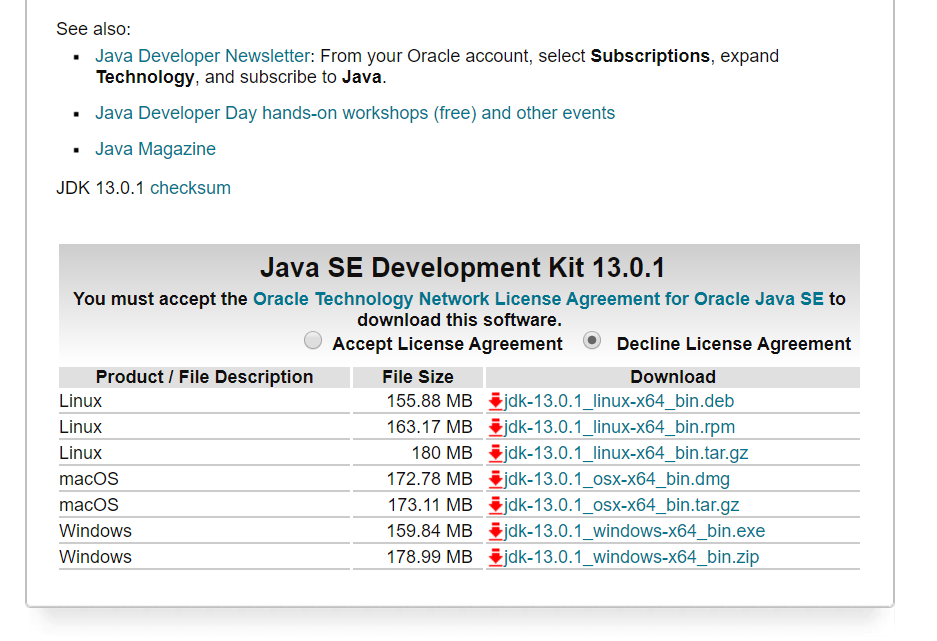
\includegraphics[width=\textwidth]{Images/javaVersionchoice.png}
\end{figure} 
\clearpage

\subsection{Set Up Java}

Set the environment variable JAVA\_HOME to the directory where you installed the jdk.
Normally the installation path will look like "C:\textbackslash Program-Files\textbackslash Java \textbackslash jdk-13.0.1" where jdk-13.0.1 could be different if you downloaded a more recent version. To set up environmente variable in windows search in the search bar of the pc "env" a choice with 
"Edit the system environment variables" or in italian " modifica le variabili di ambiente relative al sistema " should appear  
click it than click environment variable at the bottom right of the menu which appears. A new window should appear, check if the variable JAVA\_HOME is available in the list at the top, if it isn't  press add otherwise choose it and press modify. In the opened window insert as variable name JAVA\_HOME and as value the path of your jdk. After confirmation you can close all.

\begin{figure}[h]
\centering
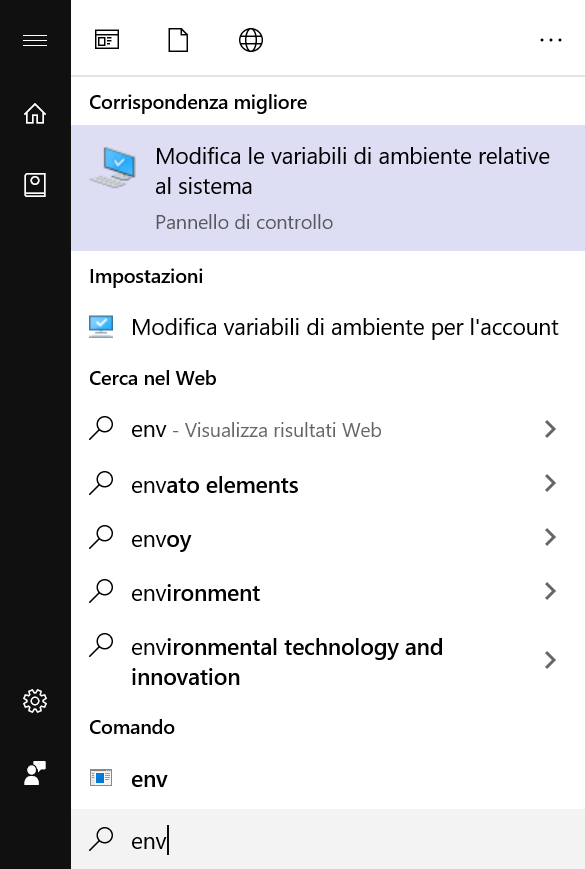
\includegraphics{Images/environment variable.png}
\end{figure} 

\begin{figure}[h]
\centering
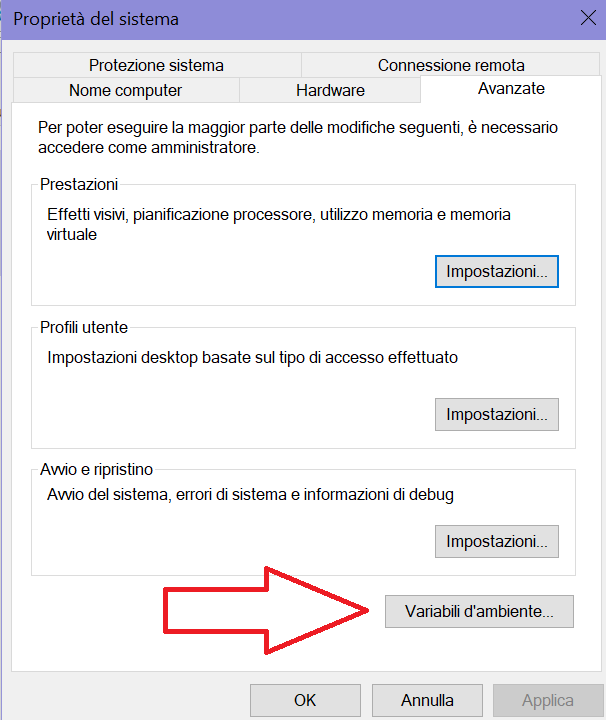
\includegraphics{Images/env.png}
\end{figure} 
\begin{figure}[h]
\centering
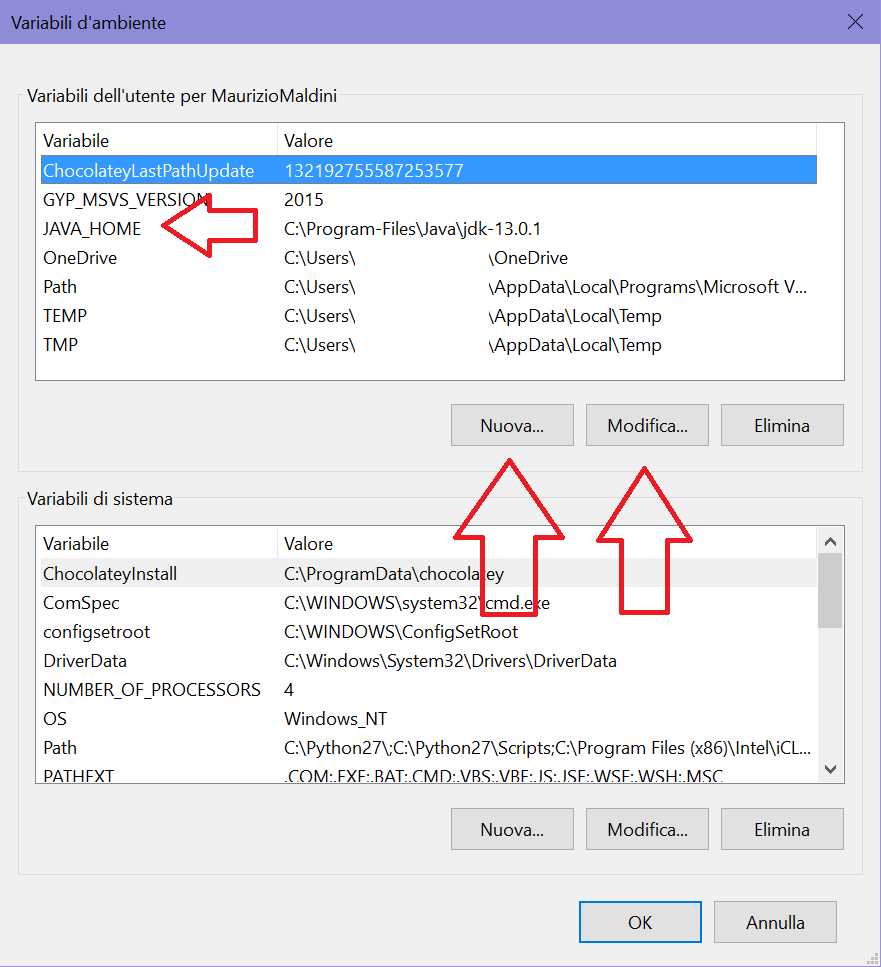
\includegraphics{Images/environment.png}
\caption{\label{fig:myi} Here you can see where java home should be visible if not available add it or update if it is outdated}
\end{figure} 

\begin{figure}[h]
\centering
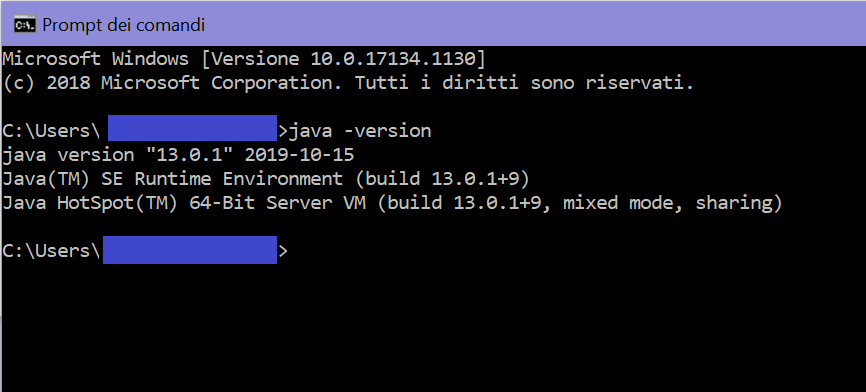
\includegraphics[width=\textwidth]{Images/javaInstallationCheck.png}
\caption{\label{fig:myi} Now go to the console (for windows in the search bar search "cmd" and open command prompt) wirte the commande java -version
you should get and output similar to this image.If you don't get a similar message check if the variable JAVA\_HOME is set correctly. If you get a different version from the one you installed check if you have other oracle products installation and check if they are not interfering with the environment.}
\end{figure} 



\clearpage
\subsection{Download Tomcat}
Visit the \href{https://tomcat.apache.org/download-90.cgi}{tomcat download page}.
Download the correct version of the binary distribution for your os. For a lightweight deployment we suggest the zip version.
Once downloaded unzip the folder. Open the folder and open the folder bin inside it, in this folder than execute the startup.bat for windows or startup.sh for linux. If java installation worked correctly and java home is set correctly you should get a screen like this one.
if you got this screen run the shutdown.bat or shutdown.sh to stop the server. If a console flashes in and disappear immediately there is an error in the java home variable.
\begin{figure}[h]
\centering
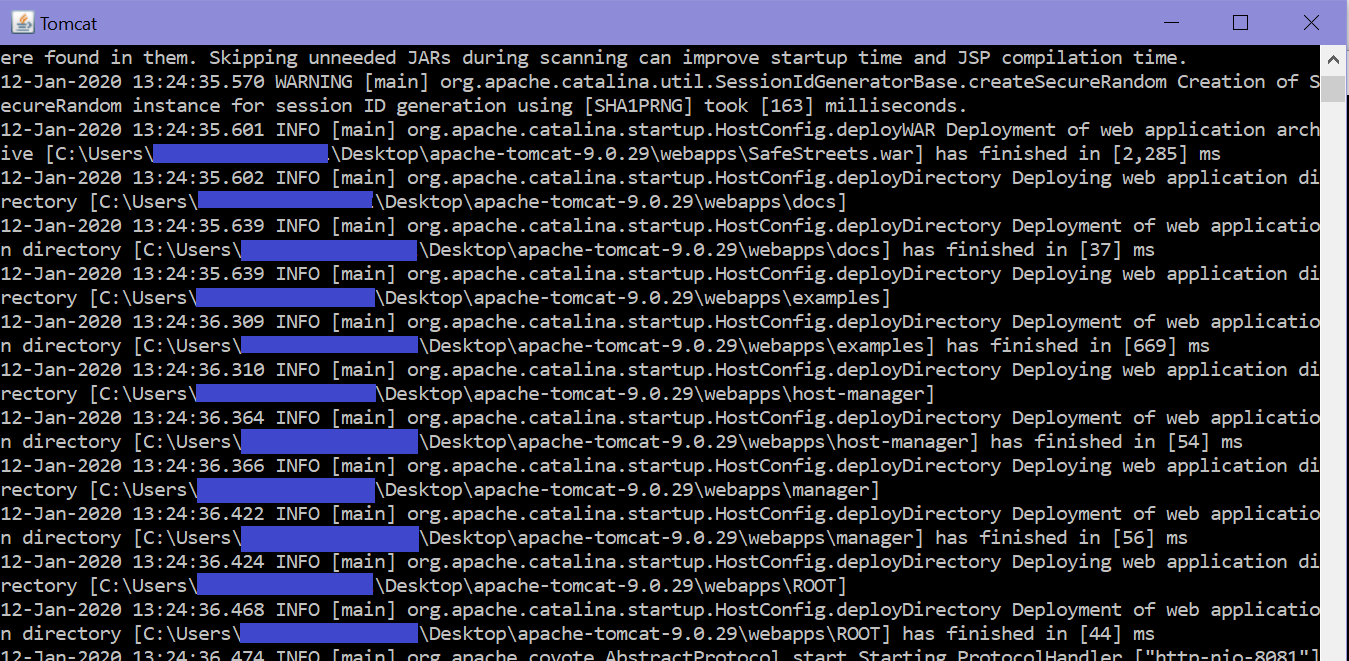
\includegraphics[width=\textwidth]{Images/tomcatStartup.png}
\end{figure} 
\clearpage
\subsection{Download MySQl}
If you have already a mysql server on your machine you may skip this part, keep in mind the server should be updated to a recent version.
Visit the \href{
https://dev.mysql.com/downloads/installer/}{MySQL insaller installation page}.
The page should show you the most appropriate installer for you operating system.
Install it and run it. The installer should show you this window after loading.
\begin{figure}[h]
\centering
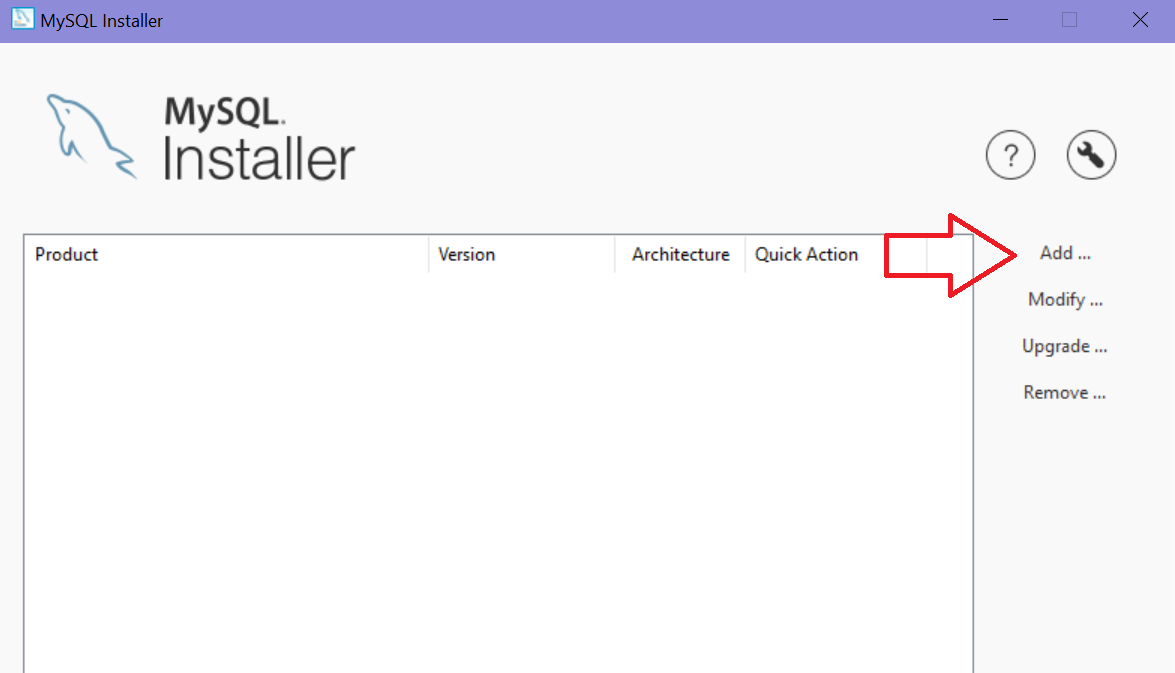
\includegraphics[width=\textwidth]{Images/mysqlinstaller.png}
\caption{\label{fig:myi} Click on the Add button}
\end{figure} 
\begin{figure}[h]
\centering
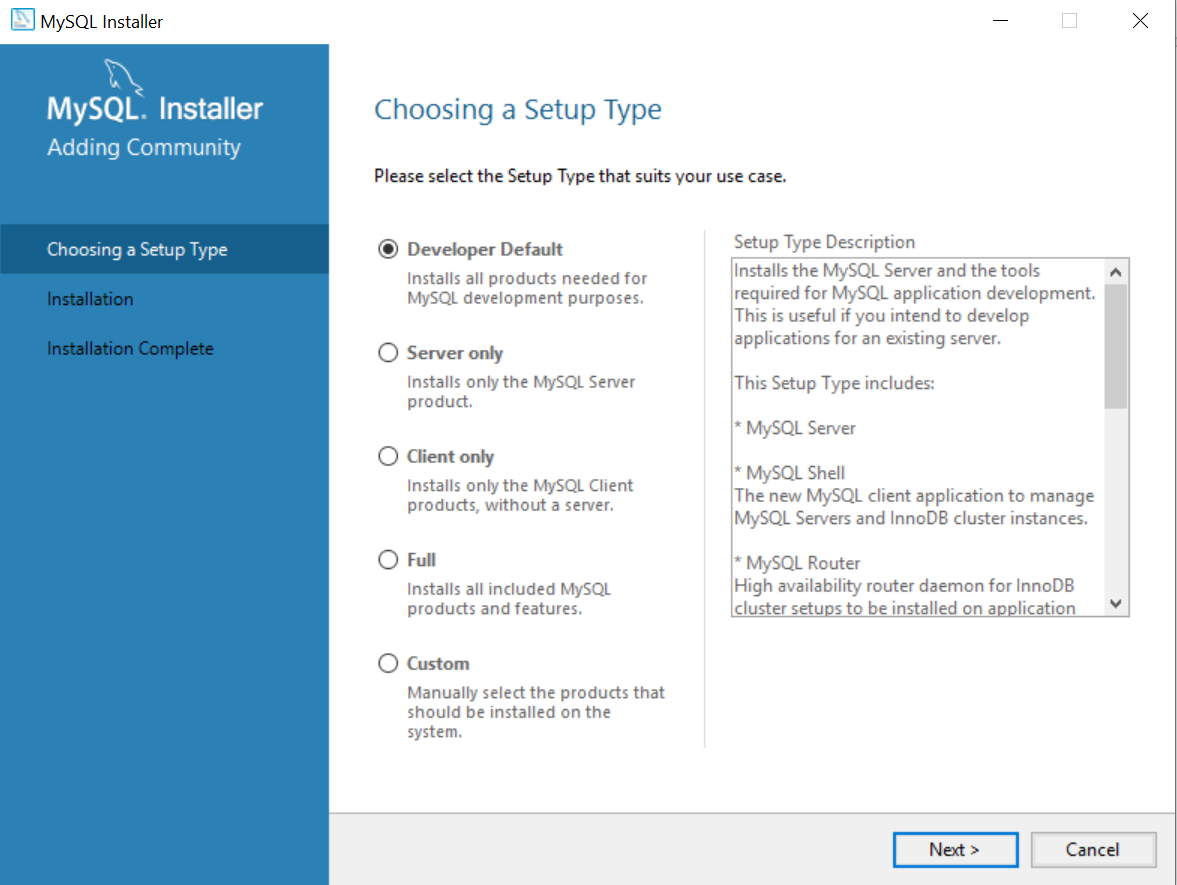
\includegraphics[width=\textwidth]{Images/mysql-download.png}
\caption{\label{fig:fmy} select Server only}
\end{figure} 
\begin{figure}[h]
\centering
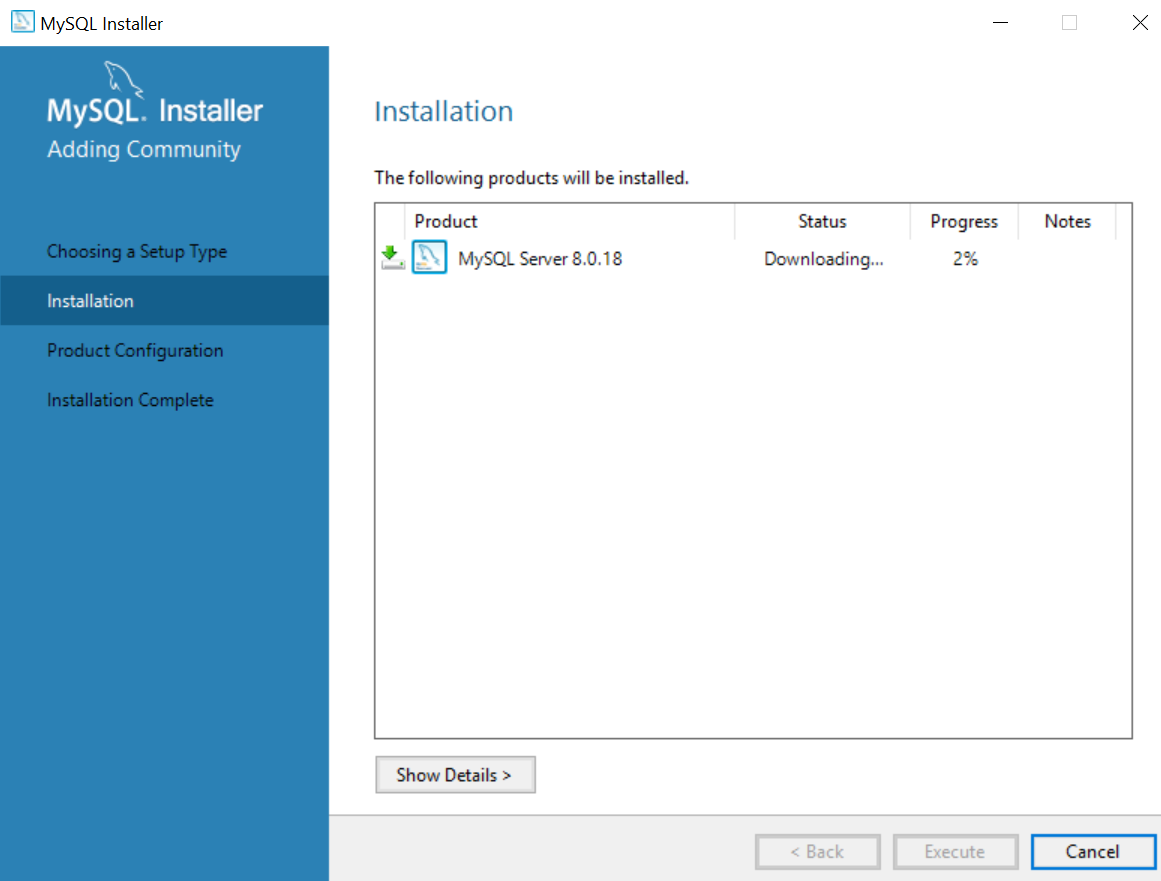
\includegraphics[width=\textwidth]{Images/mysql-downloading.png}
\caption{\label{fig:fmy} click execute. After the download is complete go to product configuration}
\end{figure} 
\begin{figure}[h]
\centering
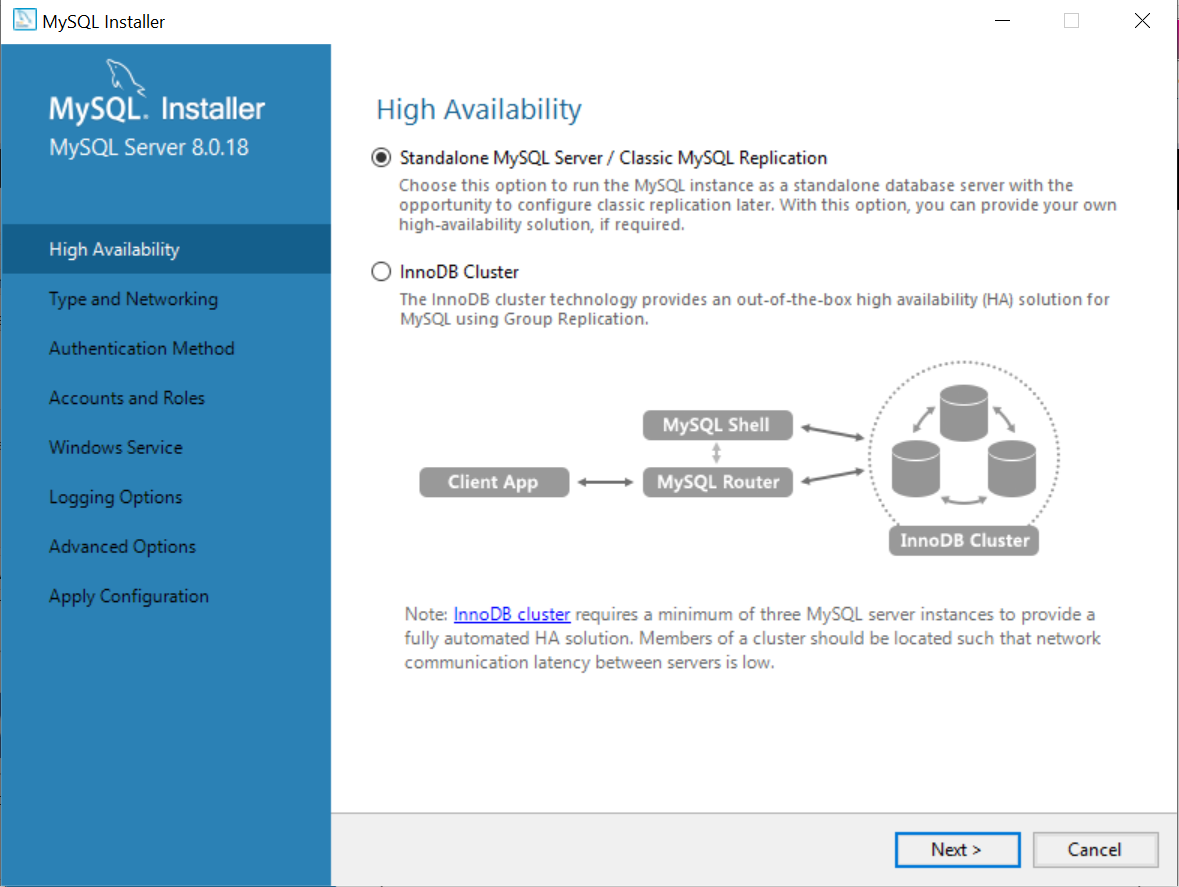
\includegraphics[width=\textwidth]{Images/first-mysql.png}
\caption{\label{fig:fmy} select Standalone MySQL Server  and then click Next }
\end{figure} 
\begin{figure}[h]
\centering
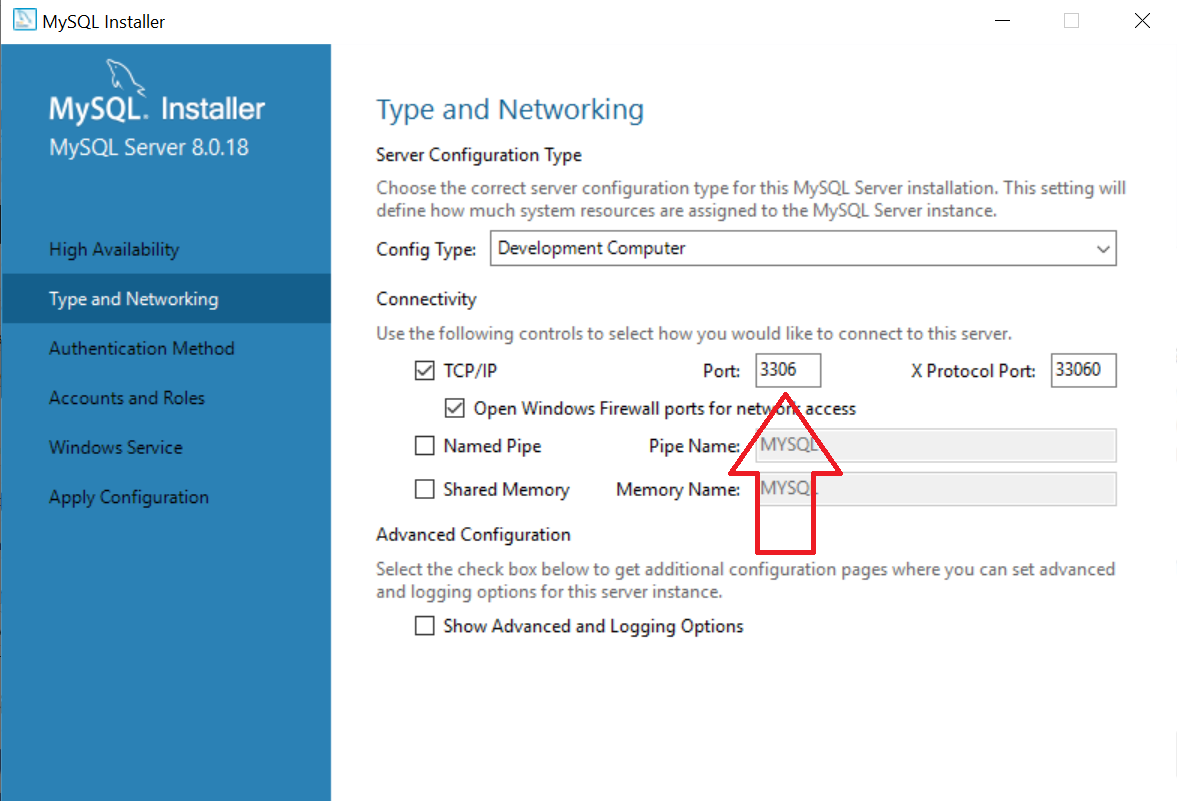
\includegraphics[width=\textwidth]{Images/second-mysql.png}
\caption{\label{fig:fmy} Check if the informations shown are the same. If you change port remember the number you insert to change later change our application setting. Click Next.Choose an authentication method. Click next.}
\end{figure} 

\begin{figure}[h]
\centering
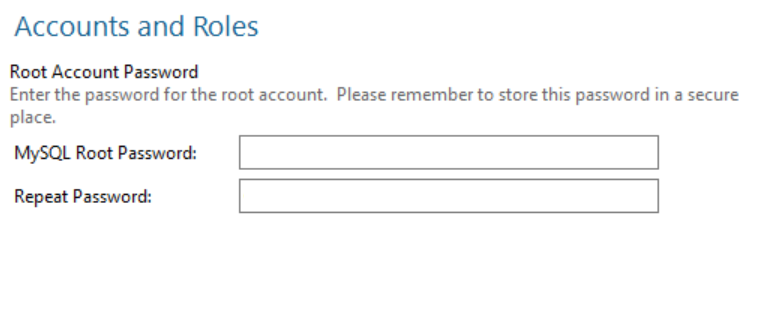
\includegraphics[width=\textwidth]{Images/4-mysql.png}
\caption{\label{fig:fmy} Set a password for the mysql server. Click next.}
\end{figure}
\begin{figure}[h]
\centering
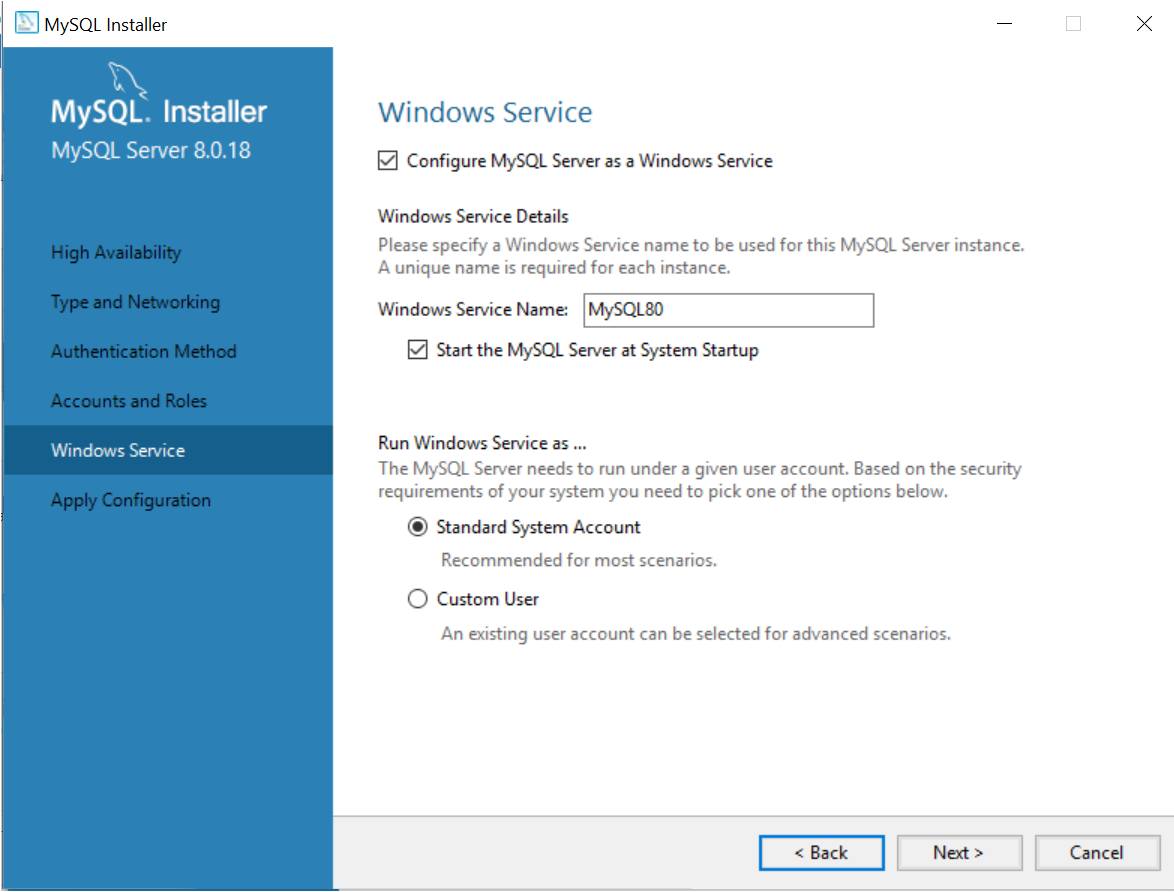
\includegraphics[width=\textwidth]{Images/6-mysql.png}
\caption{\label{fig:fmy} Click next}
\end{figure}
\begin{figure}[h]
\centering
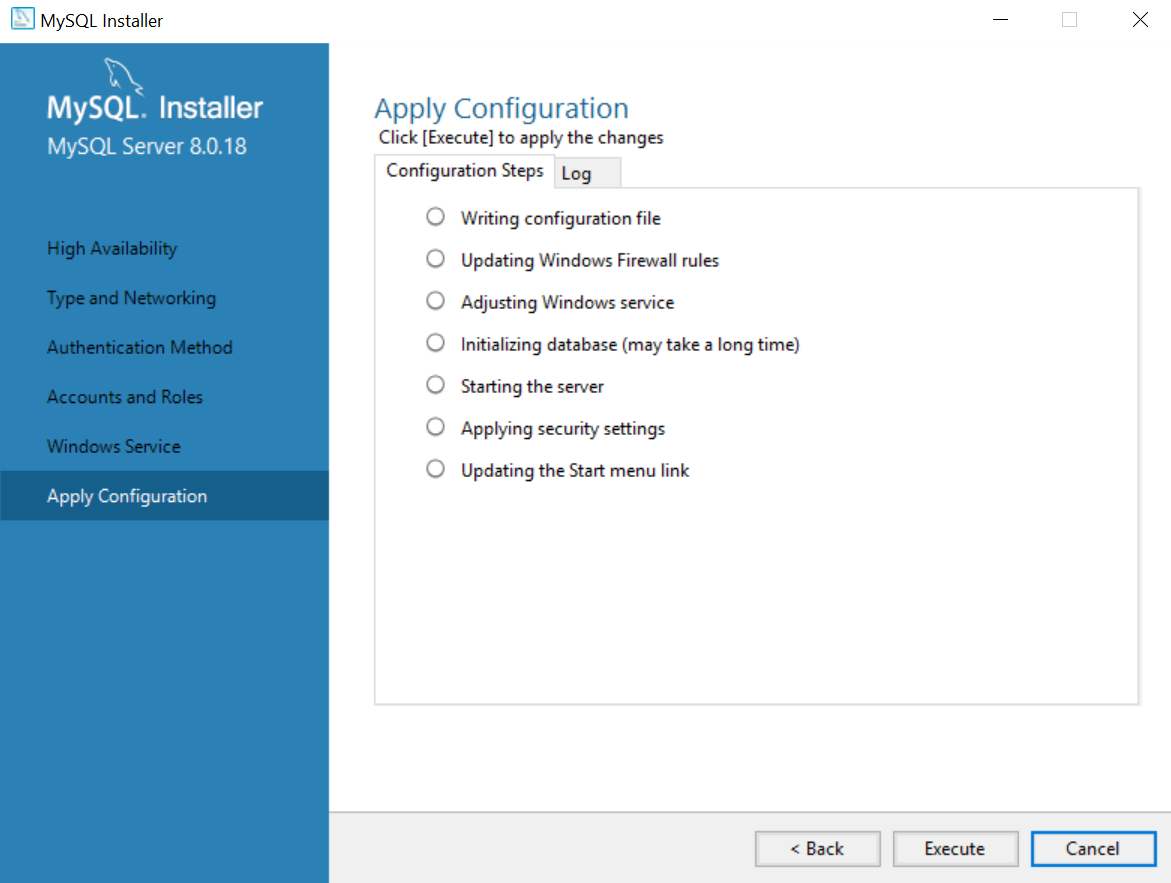
\includegraphics[width=\textwidth]{Images/7-mysql.png}
\caption{\label{fig:fmy} Click execute and after the configuration is complete click next.Your installation should be complete.
Type in your search bar mysql you should get an entry called mysql 8.0 command line client open it and insert the password you have chosen for mysql. You should now be able to use my sql server on your pc.}
\end{figure}


\clearpage
\subsection{Configure SafeStreets}
From our directory get the DB.sql file and paste it inside the bin directory that you can find inside the mysql installation forlder.
You should find the folder inside your program folder.
Now open mysql command line client. Once you log in type the commands  
\newline 
\newline create schema safestreets;
\newline use safestreets; 
\newline source DB.sql;.
\newline
\newline 
Don't forget the semicolon(;) at the end of the commands.
This should install the database. Try the command \newline select * from authority;  
\newline if a table is returned than the import is successful.

After this open the configuration.txt file in our directory.
Don't delete the text on the left part and always keep at least a white space between left part and right part.
Set the variables to the correct values. 
Set Db\_username to the username you use to connect to mysql(if you didn't choose any write root) , db\_password to the password you use to connect to the database. If you changed port for mysql server during the installation change the number 3306 with the chosen port in db\_url mail\_username and mail\_password are used to send email to the account which registers to our service. you may put there your gmail account username and password (but only if you don't have a 2 factor authentication enabled, we suggest you to keep the account which is already there)
Server Address should remain unchanged ,  if you modify tomcat configuration and change port please change it also here.
Photo path represents the path were the photos are saved. If you want change it to desired folder (which must be accessible for both read and write operations).
If you want to check what issues happens when running the code keep verbose true  otherwise change true with false. Once you modified the configuration.txt put it in the tomcat  folder.
Now put the SafeStreets.war file from our directory in the webapps folder. Now executing the startup.bat or startup.sh from the bin folder of tomcat the server should be working.
For a first check go to webapps folder and see if along with the SafeStreets app there is now a SafeStreets folder. After that open a browser search  http://localhost:8080/SafeStreets/ you should be seeing now our homepage.
On tomcat console some setup messages are shown if any error occures check out if there are errors printed there.
Whenever you want to stop the server execute the shutdown.bat or shutdown.sh in the bin folder of tomcat and the server will go oflline.
To Start testing you can get some accounts credentials executing from mysql command line the commands.
\newline 
\newline
use safestreets; 
\newline
select * from user;
\newline 
\newline
You may register as a new Citizen from the login and registration page. Other users can be registered only by other users. Authorities only by municipality. Municipality only from municipalities and Managers . Managers only by managers.
 